\motto{There are two principal ways to formulate mathematical assertions (problems, conjectures, theorems, \dots ): Russian and French. The Russian way is to
choose the most simple and specific case (so that nobody could simplify the formulation preserving the main point). The French way is to generalize the statement
as far as nobody could generalize it further.

--- Vladimir Arnold\footnote{Vladimir Igorevich Arnold (1937--2010), who became a professor at l'Université Paris IX after the dissolution of USSR, was always sick of France (so am I!). In the public lecture entitled ``Sur l'éducation mathématique'' in 1997, he invented the famous joke ``Combien font $2+3$?'' to question the French education system.}}
\chapter{Toric pluripotential theory on ample line bundles}
\label{chap:toric_ample}

This chapter develops the toric form of pluripotential theory in the case of an ample line bundle. Throughout the chapter, $P\subseteq M_{\mathbb R}$ is a full-dimensional smooth lattice polytope, $\Sigma$ is the corresponding fan, $X=X_\Sigma$ is the associated smooth projective toric variety, and $L=\mathcal O_X(D_P)$ is the ample toric line bundle defined by $P$.

The basic principle is that toric plurisubharmonic metrics on $L$ can be described by convex functions on $N_{\mathbb R}$. Under this dictionary, singularity type, rooftop envelopes, Monge--Amp\`ere mass and energy all admit convex-analytic interpretations. The Newton body of a toric potential is the main invariant in this chapter: it records the effective convex domain seen by multiplier ideals and non-pluripolar mass.

The central result is Yao's theorem, stated as \cref{thm:Yao}. It characterizes the torus characters belonging to multiplier-ideal spaces in terms of the Newton body. As a consequence, the asymptotic dimension of
\[
    \mathrm{H}^0\left(X,L^k\otimes\mathcal I(k\varphi)\right)
\]
is governed by the Euclidean volume of the Newton body. This gives a toric model for the general volume theorem proved later in \cref{chap:Igood} and shows, in the ample toric setting, why multiplier ideals and non-pluripolar mass should be related.

The chapter also proves the real Monge--Amp\`ere formula for toric metrics, the toric energy formula, and the expression of the $d_1$-distance in convex terms. These results will be used again in \cref{chap:toric_big}, where the ample assumption is removed and the Newton body is compared with partial Okounkov bodies.

We assume familiarity with basic toric geometry at the level of \cite{CLS11}. Some convex-analytic facts used below are recalled in \cref{chap:convex}. The chapter can be skipped on a first reading if the reader is only interested in the non-toric theory, but it provides useful examples and a guiding model for several later constructions.

Finally, throughout the book convex functions are understood in the usual sense: the function $\mathbb R\ni x\mapsto x^2$ is convex. This convention is opposite to the convention often used in toric geometry, including parts of \cite{CLS11}; care is therefore needed when comparing formulas.

\section{Toric setup}\label{sec:toricsetup}
Let $T$ be a complex torus of dimension $n$\footnote{Namely, an algebraic group defined over $\mathbb{C}$, which is isomorphic to $\mathbb{G}_{\mathrm{m}}^n$.} and let $T_c\subseteq T(\mathbb{C})$ denote the corresponding compact torus.

Write $M$ for the character lattice of $T$, which is a free Abelian group of rank $n$. Similarly, let $N$ be the cocharacter lattice of $T$, which is the dual lattice of $M$. Given $m\in M$, the corresponding character of $T$ is denoted by $\chi^m$.
Write $M_{\mathbb{R}}=M\otimes_{\mathbb{Z}} \mathbb{R}$ and $N_{\mathbb{R}}=N\otimes_{\mathbb{Z}}\mathbb{R}$. The pairing between $M_{\mathbb{R}}$ and $N_{\mathbb{R}}$ is denoted by $\langle \bullet,\bullet \rangle$.

Let $P\subseteq M_{\mathbb{R}}$ be a full-dimensional \emph{smooth}\footnote{Recall that \emph{smooth} means that for every vertex $v\in P$, if $w_E$ denotes the first lattice point after $v$ as one traverses each edge $E$ of $P$ containing $v$, then $\{w_E-v\}_E$ forms a basis of $M$. See \cite[Definition~2.4.2]{CLS11}. We also say $P$ is a \emph{Delzant polytope}\index{polytope!Delzant polytope} in this case.} lattice polytope\footnote{A \emph{lattice polytope}\index{polytope!lattice polytope} in $M_{\mathbb{R}}$ is the convex hull of finitely many points in $M$.}.

Given any (closed) facet $F$ of $P$, let $u_F\in N$ denote the unique ray generator (the first non-zero integral element) of the inward normal ray of $F$. Then $P$ can be represented as
\begin{equation}\label{eq:Pfacetrep}
P=\left\{m\in M_{\mathbb{R}}: \langle m,u_F \rangle\geq -a_F\textup{ for all facets }F\textup{ of } P\right\}
\end{equation}
for some uniquely determined integers $a_F$. The presentation is called the \emph{facet presentation}\index{polytope!facet presentation} of $P$.

Given any (closed) face $Q$ of $P$, we let $\sigma_Q\subseteq N_{\mathbb{R}}$ be the closed convex cone generated by the $u_F$'s, where $F$ runs over all facets of $P$ containing $Q$. When $Q=P$, $\sigma_P$ is understood as $\{0\}$.

Let $\Sigma$ be the \emph{(inner) normal fan}\index{fan!normal fan of a polytope} of $P$. Namely,
\[
\Sigma=\left\{\sigma_Q:Q\textup{ is a face of }P\right\}.
\]
The notation $\Sigma(1)$ denotes the set of rays in $\Sigma$. Note that $\Sigma(1)$ is in bijective correspondence with the set of facets of $P$. In fact, given any facet $F$ of $P$, the cone $\sigma_F$ is just the ray generated by $u_F$, namely, the inward normal ray of $F$.

For any $\rho\in \Sigma(1)$, let $u_{\rho}\in N$ denote the ray generator of $\rho$, namely the first non-zero element in $N\cap \rho$. If $\rho=\sigma_F$ for some facet $F$ of $P$, then $u_{\rho}=u_F$.

Now the facet presentation \eqref{eq:Pfacetrep} can be equivalently rewritten as
\[
P=\left\{m\in M_{\mathbb{R}} : \langle m,u_{\rho} \rangle\geq -a_{\rho}\textup{ for all }\rho\in \Sigma(1) \right\}.
\]
Let $\Supp_P\colon N_{\mathbb{R}} \rightarrow \mathbb{R}$ denote the \emph{support function} of $P$. Recall that the support function (\cref{ex:suppfun}) of $P$ is defined as
\[
\Supp_P(n)=\max\left\{ \langle m,n \rangle: m\in P \right\}.
\]
Note that our support function differs from \cite[Proposition~4.2.14]{CLS11}, where instead of a maximum, they took the minimum.

Recall that the \emph{characteristic function} $\chi_P\colon M_{\mathbb{R}}\rightarrow \{0,\infty\}$ of $P$ is defined as in \cref{ex:charconvex}:
\[
\chi_P(m)\coloneqq
    \begin{cases}
        0,&\quad m\in P;\\
        \infty,&\quad m\not\in P.
    \end{cases}
\]

Let $X=X_{\Sigma}$ be the smooth projective toric variety corresponding to $\Sigma$. See \cite[Theorem~3.1.5]{CLS11} for the construction of $X$ and \cite[Theorem~3.1.19]{CLS11} for the smoothness of $X$. There is a canonical embedding $T\subseteq X$ as a dense Zariski open subset.

Let $D$ be the Cartier divisor on $X$ defined by $P$:
\[
D=\sum_{\rho\in \Sigma(1)} a_{\rho}D_{\rho},
\]
where $D_{\rho}$ is the toric prime divisor defined by $\rho$ under the orbit-cone correspondence \cite[Theorem~3.2.6]{CLS11}.

Let $L$ be the toric line bundle induced by $P$, namely $L=\mathcal{O}_X(D)$. Since $P$ is a smooth (Delzant) lattice polytope, $L$ is very ample by \cite[Proposition~2.4.4, Proposition~6.1.10]{CLS11}; in particular, $L$ is ample.

We will choose the base $\mathrm{e}$ for the logarithm map
\begin{equation}\label{eq:log}
\mathbb{C}^*\rightarrow \mathbb{R},\quad z\mapsto \log|z|^2.\footnotemark
\end{equation}
\footnotetext{Be careful when you compare with other references, some people prefer $\log |z|$, $-\log |z|$ or $-\log |z|^2$ instead.}
This choice is fixed throughout the book. We have a canonical identification
\[
T(\mathbb{C})=\mathrm{Hom}(M,\mathbb{C}^*)\xlongrightarrow{\sim} N\otimes_{\mathbb{Z}}\mathbb{C}^*.
\]
The logarithm map then induces a tropicalization map after tensoring with $N$:
\begin{equation}
\Trop\colon T(\mathbb{C})\rightarrow N_{\mathbb{R}},\quad p\mapsto \left( M \ni m\mapsto \log \left|\chi^m(p)\right|^2 \right).
\end{equation}
\index{$\Trop$}

Before proceeding, it is always helpful to understand everything in our favorite example.
\begin{example}\label{ex:P1toric}
    We take $n=1$ and $P=[0,1]\subseteq M_{\mathbb{R}}=\mathbb{R}$. In this case, the facet representation \eqref{eq:Pfacetrep} becomes
    \[
    P=\bigl\{m\in \mathbb{R}: \langle m,1 \rangle \geq 0, \langle m,-1 \rangle \geq -1\bigr\},
    \]
    with $u_{\{0\}}=1$, $u_{\{1\}}=-1$, $a_{\{0\}}=0$ and $a_{\{1\}}=1$. The normal fan $\Sigma$ is
    \[
    \Sigma=\bigl\{(-\infty,0], \{0\}, [0,\infty) \bigr\}.
    \]
    See \cref{fig:fanP1}.
        \begin{figure}[ht]
        \centering
        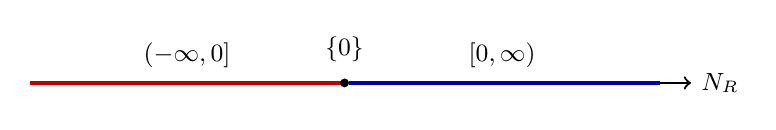
\begin{tikzpicture}[scale=1.0, line width=0.6pt, every node/.style={font=\small}]
          % Real line N_R = R drawn with the two rays in colour, directly on the axis
          \draw[red!75!black, line width=1.4pt] (-4.0, 0) -- (-0.05, 0);
          \draw[blue!70!black, line width=1.4pt] (0.05, 0) -- (4.0, 0);
          \draw[thick, ->] (4.0, 0) -- (4.4, 0) node[right, black] {$N_{\mathbb{R}}$};
          % Origin (the 0-dim cone {0})
          \fill (0,0) circle (1.6pt);
          % Labels above the line
          \node[above=2pt] at (-2.0, 0) {$(-\infty,0]$};
          \node[above=4pt] at (0, 0) {$\{0\}$};
          \node[above=2pt] at (2.0, 0) {$[0,\infty)$};
        \end{tikzpicture}
        \caption{The fan $\Sigma$ of $\mathbb{P}^1$ in $N_{\mathbb{R}}=\mathbb{R}$, consisting of the two rays $(-\infty,0]$, $[0,\infty)$ and the cone $\{0\}$.}
        \label{fig:fanP1}
    \end{figure}

    The corresponding toric variety is just $X=\mathbb{P}^1$. Under the orbit-cone correspondence, we have
    \[
    D_{[0,\infty)}=[0],\quad D_{(-\infty,0]}=[\infty].
    \]
    The associated divisor $D=[\infty]$ and therefore,
    \[
    L=\mathcal{O}_X(D)=\mathcal{O}_{\mathbb{P}^1}(1).
    \]
\end{example}


\section{Toric plurisubharmonic functions}\label{sec:tpf}

We continue to use the notations of \cref{sec:toricsetup}.

\begin{lemma}\label{lma:convextopsh}
    Let $F\colon N_{\mathbb{R}}\rightarrow [-\infty,\infty]$ be a function. Then the following are equivalent:
    \begin{enumerate}
        \item\label{itm:lma:convextopsh:1} $F$ is convex and takes values in $\mathbb{R}$, and
        \item\label{itm:lma:convextopsh:2} $\Trop^*F$ is plurisubharmonic on $T(\mathbb{C})$.
    \end{enumerate}
\end{lemma}
\begin{proof}
We may choose an identification $N\cong \mathbb{Z}^n$ so that we have an identification $T(\mathbb{C})\cong \mathbb{C}^{*n}$.
Then $\Trop$ is identified with the map
\[
\Trop\colon \mathbb{C}^{*n}\rightarrow \mathbb{R}^n,\quad (z_1,\ldots,z_n)\mapsto \left(\log|z_1|^2,\ldots,\log|z_n|^2\right).
\]

\ref{itm:lma:convextopsh:1} $\implies$ \ref{itm:lma:convextopsh:2}. By the standard convolution regularization of finite convex functions, let $F_k\in C^{\infty}(\mathbb{R}^n)\cap \Conv(\mathbb{R}^n)$ be a decreasing sequence with limit $F$. It follows from a straightforward computation that
    \begin{equation}\label{eq:ddctrop}
    \begin{split}
    \ddc \Trop^*F_k(z_1,\ldots,z_n)
    =&\frac{\mathrm{i}}{2\pi} \sum_{i,j=1}^n \partial_{ij}F_k\left(\log|z_1|^2,\ldots,\log|z_n|^2\right)\\
    &\times z_i^{-1}\overline{z_j}^{-1}\mathrm{d}z_i\wedge \mathrm{d}\overline{z_j}.
    \end{split}
    \end{equation}
    So $\Trop^* F_k$ is plurisubharmonic. It follows from \cref{prop:pshfunction_closedseq} that $\Trop^* F$ is plurisubharmonic.

\ref{itm:lma:convextopsh:2} $\implies$ \ref{itm:lma:convextopsh:1}. It follows from \cref{lma:invariantpshfunfinite} that $F$ is finite. Moreover, by radial regularization, we may find a decreasing sequence $\varphi_k$ of $(S^1)^n$-invariant smooth psh functions on $\mathbb{C}^{*n}$ with limit $\Trop^*F$. Write $\varphi_k=\Trop^* F_k$ for some function $F_k\colon \mathbb{R}^n\rightarrow \mathbb{R}$; it follows from \eqref{eq:ddctrop} that $F_k$ is convex for all $k$. Therefore, $F$ is convex by \cref{lma:convdecnet}.
\end{proof}

Next we define a canonical K\"ahler form in $c_1(L)$.

Let $G_0\colon M_{\mathbb{R}}\rightarrow (-\infty,\infty]$ be defined as
\begin{equation}\label{eq:G0def}
G_0(m)\coloneqq
\begin{cases}
\sum\limits_{\rho \in \Sigma(1)} \left(\langle m, u_{\rho}\rangle +a_{\rho}\right)\log  \left(\langle m, u_{\rho}\rangle +a_{\rho}\right)\footnotemark,&\textup{if }m\in P,\\
\infty,& \textup{otherwise}.
\end{cases}
\end{equation}
\footnotetext{We understand that $0\log 0=0$ in this expression.}

This is a closed proper convex function and $G_0\sim \chi_P$, where $\sim$ is the relation defined in \cref{def:partialorderconv}.

Let
\begin{equation}\label{eq:F0def}
F_0=G_0^* \in \mathcal{E}^{\infty}(N_{\mathbb{R}},P).
\end{equation}
Here $G_0^*$ is the Legendre transform of $G_0$, as recalled in \cref{def:Legendregeneral}. The set $\mathcal{E}^{\infty}(N_{\mathbb{R}},P)$ is defined in \cref{def:convexPfunctions}.

By Guillemin's theorem \cite{Gui94, CDG03}, $\ddc\Trop^* F_0$ can be extended to a unique K\"ahler form $\omega$ in $c_1(L)$. The K\"ahler form $\omega$ is clearly $T_c$-invariant.

For each $\rho\in \Sigma(1)$, we write
\[
    r_{\rho}(m)=\log \left(\langle m,u_{\rho}\rangle +a_{\rho}\right)+1,\quad m\in P.
\]
It follows from \eqref{eq:G0def} that
\begin{equation}\label{eq:nablaG0}
    \nabla G_0(m)=\sum_{\rho\in \Sigma(1)} r_{\rho}(m)u_{\rho},\quad m\in \Int P.
\end{equation}


\begin{example}\label{ex:P1toric1}
Let us move on with our favorite example \cref{ex:P1toric}. We continue to use the same notations. In this case,
\[
G_0(m)=
\begin{cases}
    m\log m+(1-m)\log (1-m),& \textup{if } m\in [0,1],\\
    \infty,&\textup{otherwise}.
\end{cases}
\]
The Legendre transform is given\footnote{While reading an advanced mathematical textbook/paper, I usually tend to trust the authors for their elementary computations. A few years ago, I was asked to present the result of a landmark paper written by two respected mathematicians on a conference. After spending a few days on the elementary integrals, I found out that all non-trivial constants in that paper were wrong. So I ask the readers to really verify this expression, if it is not obvious to you.} by
\[
F_0(n)=\log\left(1+\mathrm{e}^n\right).
\]
Composing with the tropicalization map, we find that
\[
\omega|_{\mathbb{C}^*}(z)=\ddc\log\left(1+|z|^2\right).
\]
This is exactly the Fubini--Study metric as we have seen in \cref{ex:LPP1}.

We can now explain one subtlety: in our expression \eqref{eq:G0def}, there is no factor $1/2$ before the sum; the absence of the factor $1/2$ matches the choice $\Trop(z)=\log|z|^2$ rather than $\log|z|$ in our tropicalization map \eqref{eq:log}.
\end{example}


Let $\PSH_{\tor}(X,\omega)$\index{$\PSH_{\tor}(X,\omega)$} denote the set of $T_c$-invariant $\omega$-psh functions.
\begin{theorem}\label{thm:toricpsh}
    There are canonical bijections between the following three sets:
    \begin{enumerate}
        \item\label{itm:thm:toricpsh:1} The set of $\varphi\in \PSH_{\tor}(X,\omega)$,
        \item\label{itm:thm:toricpsh:2} the set $\mathcal{P}(N_{\mathbb{R}},P)$ in \cref{def:convexPfunctions}, namely, the set of convex functions $F\colon N_{\mathbb{R}}\rightarrow \mathbb{R}$ satisfying $F\preceq \Supp_P$, and
        \item\label{itm:thm:toricpsh:3} the set of closed proper convex functions $G\in \Conv(M_{\mathbb{R}})$ satisfying
        \[
        G|_{M_{\mathbb{R}}\setminus P}\equiv \infty.
        \]
    \end{enumerate}
\end{theorem}
For the notions of closedness and properness, we refer to \cref{def:convexfun} and \cref{def:convexclosure}.

\begin{proof}
The bijection between \ref{itm:thm:toricpsh:2} and \ref{itm:thm:toricpsh:3} is the classical Legendre duality. Given $F$ as in \ref{itm:thm:toricpsh:2}, we construct $G=F^*$ and \emph{vice versa}, see \cref{prop:Fsuppchar}.

The map from \ref{itm:thm:toricpsh:1} to \ref{itm:thm:toricpsh:2} is given as follows: Given $\varphi\in \PSH_{\tor}(X,\omega)$, since $\varphi$ is $T_c$-invariant, we can find $f\colon N_{\mathbb{R}}\rightarrow [-\infty,\infty)$ such that
\begin{equation}\label{ex:varphitropf}
\varphi|_{T(\mathbb{C})}=\Trop^*f.
\end{equation}
We then define $F=f+F_0$. Then $\Trop^* F\in \PSH(T(\mathbb{C}))$.
By \cref{lma:convextopsh}, $F(n)$ is finite for any $n\in N_{\mathbb{R}}$ and $F$ is convex. Moreover, $F\preceq \Supp_P$ since $\varphi$ is bounded from above on the compact space $X$ and $F_0\preceq \Supp_P$.

Conversely, given a map $F\in \mathcal{P}(N_{\mathbb{R}},P)$, then
\[
\Trop^*(F-F_0)\in \PSH\left(T(\mathbb{C}),\omega|_{T(\mathbb{C})}\right).
\]
Since $F\preceq \Supp_P$ and $F_0\sim \Supp_P$, the difference $F-F_0$ is bounded from above. Hence the corresponding local psh potentials are locally bounded from above near $X\setminus T(\mathbb{C})$. It follows from \cref{thm:GRexten} that this function can be extended uniquely to an $\omega$-psh function on $X$. The uniqueness of the extension guarantees its $T_c$-invariance.

The two maps are inverse to each other by construction.
\end{proof}


Given $\varphi\in \PSH_{\tor}(X,\omega)$, we will write $F_{\varphi}$ and $G_{\varphi}$ for the convex functions given by \cref{thm:toricpsh}. From the proof, we have the following relations:
\begin{equation}\label{eq:FvarphidefGdef}
\varphi|_{T(\mathbb{C})}=\Trop^*\left(F_{\varphi}-F_0\right),\quad G_{\varphi}=F_{\varphi}^*.
\end{equation}
In particular, $\varphi|_{T(\mathbb{C})}$ is locally bounded. We will frequently use this result without further explanation.

\begin{example}\label{ex:FGsimplevarphi}
    Let us take our favorite example \cref{ex:P1toric1} again. We will continue to use the same notations.

    Recall that in \cref{ex:logsingP1} and \cref{ex:loglogsing}, we constructed two $S^1$-invariant functions in $\PSH(X,\omega)$.

    We begin with the function $\varphi$ in \cref{ex:logsingP1}. Recall that
    \[
    \varphi(z)=\log \frac{|z|^2}{|z|^2+1}
    \]
    for $z\in \mathbb{C}$. The function $f\colon \mathbb{R}\rightarrow \mathbb{R}$ in \eqref{ex:varphitropf} is therefore
    \[
    f(n)=\log \frac{\mathrm{e}^{n}}{1+\mathrm{e}^{n}}.
    \]
    Therefore, $F_{\varphi}\colon \mathbb{R}\rightarrow \mathbb{R}$ is
    \[
    F_{\varphi}(n)=n.
    \]
    Correspondingly, $G_{\varphi}\colon \mathbb{R}\rightarrow \mathbb{R}$ is
    \[
    G_{\varphi}(m)=
    \begin{cases}
        0,&\textup{if } m=1;\\
        \infty,&\textup{otherwise}.
    \end{cases}
    \]

    Similarly, if $\psi$ denotes the function in \cref{ex:loglogsing}, then the function $f$ in \eqref{ex:varphitropf} is
    \[
    f(n)=
    \begin{cases}
        -\log \left(\mathrm{e}^n+1 \right)+(-\log (-n))\lor (n+2),&\textup{if } n<-\log 2;\\
        2+\log \frac{\mathrm{e}^{n}}{1+\mathrm{e}^{n}},&\textup{otherwise}.
    \end{cases}
    \]
    Therefore,
    \[
    F_{\psi}(n)=
    \begin{cases}
        (-\log (-n))\lor (n+2),&\textup{if } n<-\log 2;\\
        2+n,&\textup{otherwise}.
    \end{cases}
    \]
    The Legendre transform is tricky to compute. Let $\lambda$ be the large solution of $\log x=x-2$. So $\lambda\approx 3.146$. The smaller solution is around $0.159<\log 2\approx 0.693$. It might be helpful to have a look at the poorly drawn picture \cref{fig:logx}.

    \begin{figure}[ht]
\centering
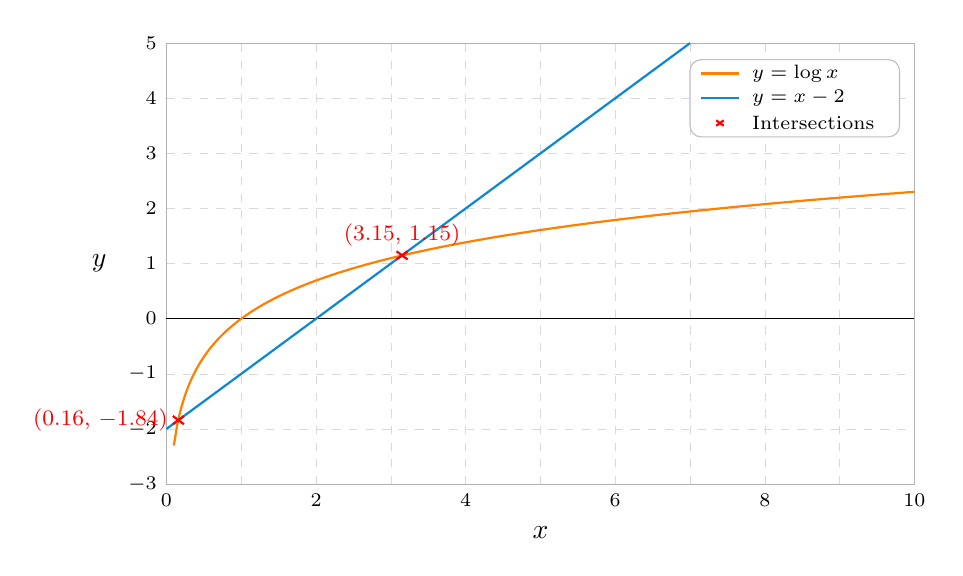
\begin{tikzpicture}[xscale=0.95, yscale=0.7]
  % Background grid
  \draw[step=1, gray!30, dashed, very thin] (0,-3) grid (10,5);
  % Bounding rectangle
  \draw[gray!60] (0,-3) rectangle (10,5);
  % x-axis line
  \draw[thin] (0,0) -- (10,0);
  % Tick labels
  \foreach \tx in {0,2,4,6,8,10}
    \node[below] at (\tx,-3) {\scriptsize $\tx$};
  \foreach \ty in {-3,-2,-1,0,1,2,3,4,5}
    \node[left] at (0,\ty) {\scriptsize $\ty$};
  % Axis labels
  \node[below] at (5,-3.6) {$x$};
  \node at (-0.9, 1) {$y$};
  % y = log(x)
  \draw[orange, thick, smooth] plot[domain=0.1:10, samples=200] (\x, {ln(\x)});
  % y = x - 2
  \draw[cyan!70!blue, thick] (0,-2) -- (7,5);
  % Intersection markers
  \draw[red, thick] plot[only marks, mark=x, mark size=3pt]
    coordinates {(3.15,1.15) (0.16,-1.84)};
  \node[red, anchor=south, font=\footnotesize, inner sep=1pt]
    at (3.15,1.25) {$(3.15,\,1.15)$};
  \node[red, anchor=east, font=\footnotesize, inner sep=2pt]
    at (0.1,-1.84) {$(0.16,\,-1.84)$};
  % Legend (top-right)
  \begin{scope}[shift={(7.1, 4.0)}]
    \draw[gray!50, fill=white, rounded corners] (-0.1,-0.7) rectangle (2.7,0.7);
    \draw[orange, thick] (0.05, 0.45) -- (0.55, 0.45);
    \node[anchor=west, font=\scriptsize] at (0.6, 0.45) {$y = \log x$};
    \draw[cyan!70!blue, thick] (0.05, 0.0) -- (0.55, 0.0);
    \node[anchor=west, font=\scriptsize] at (0.6, 0.0) {$y = x-2$};
    \draw[red, thick] plot[only marks, mark=x, mark size=2pt]
      coordinates {(0.3,-0.45)};
    \node[anchor=west, font=\scriptsize] at (0.6, -0.45) {Intersections};
  \end{scope}
\end{tikzpicture}
\caption{The graphs of $\log x$ and $x-2$.}
\label{fig:logx}
\end{figure}

It is immediate that $G_{\psi}(m)=\infty$ unless $m\in [0,1]$. Let us assume that $m\in [0,1]$. Then
\[
\begin{aligned}
G_{\psi}(m)=&\sup_{n\in \mathbb{R}} \left( mn-F_{\psi}(n)\right)\\
=& \sup_{n<-\log 2} \left( mn-(-\log (-n))\lor (n+2)\right)  \lor \sup_{n\geq -\log 2} (mn-n-2)\\
=& \sup_{n>\log 2} \left( -mn+(\log n)\land (n-2)\right)  \lor \left((1-m)\log 2-2\right).
\end{aligned}
\]
Let us focus on the first part, which can be decomposed further into
\[
\begin{aligned}
& \sup_{n>\log 2} \left( -mn+(\log n)\land (n-2)\right)\\
=& \sup_{n\in \left(\log 2,\lambda\right]} (n-2-mn) \lor \sup_{n>\lambda} (\log n-mn)\\
=& \left( (1-m)\lambda-2 \right) \lor \sup_{n>\lambda} \left(\log n-mn\right).
\end{aligned}
\]
The latter part can be computed easily:
\[
\sup_{n>\lambda} \left(\log n-mn\right)=
\begin{cases}
    -\log m-1,&\textup{if } m\in \left(0,\lambda^{-1}\right];\\
    \log \lambda -m\lambda,& \textup{if }m\in \left(\lambda^{-1},1\right].
\end{cases}
\]
Putting everything together, we find
\[
G_{\psi}(m)=
\begin{cases}
    (-\log m-1)\lor \left( (1-m)\lambda-2 \right) ,&\textup{if } m\in \left(0,\lambda^{-1}\right];\\
    (\log \lambda -m\lambda)\lor \left( (1-m)\lambda-2 \right),& \textup{if }m\in \left(\lambda^{-1},1\right].
\end{cases}
\]
This can be further simplified, the final result is
\[
G_{\psi}(m)=
\begin{cases}
    -\log m-1 ,&\textup{if } m\in \left(0,\lambda^{-1}\right];\\
    (1-m)\lambda-2 ,& \textup{if }m\in \left(\lambda^{-1},1\right];\\
    \infty,&\textup{otherwise}.
\end{cases}
\]
The graph of $G_{\psi}$ on $(0,1]$ is sketched in \cref{fig:Gpsi}.
\begin{figure}[ht]
\centering
\begin{tikzpicture}[scale=1.0, line width=0.6pt, every node/.style={font=\small}]
  % Axes (figure scale: x_fig = 5 m, y_fig = 1.5 G_psi(m))
  \draw[->, thick] (-0.4,0) -- (6.0,0) node[right] {$m$};
  \draw[->, thick] (0,-3.6) -- (0,4.4);
  % m-axis ticks at lambda^{-1} (x_fig = 1.589) and 1 (x_fig = 5)
  \draw[thin] (1.589,0.08) -- (1.589,-0.08);
  \node[anchor=north, inner sep=2pt] at (1.589,-0.08) {$\lambda^{-1}$};
  \draw[thin] (5,0.08) -- (5,-0.08);
  \node[anchor=north west, inner sep=2pt] at (5.05,-0.08) {$1$};
  % G-axis ticks at lambda - 3 (y_fig = 0.219) and -2 (y_fig = -3)
  \draw[thin] (0.08,0.219) -- (-0.08,0.219);
  \node[anchor=east, inner sep=3pt] at (-0.08,0.219) {$\lambda-3$};
  \draw[thin] (0.08,-3) -- (-0.08,-3);
  \node[anchor=east, inner sep=3pt] at (-0.08,-3) {$-2$};
  % Dashed guides at the kink point and at (1,-2)
  \draw[gray, dashed, thin] (1.589,0)
    -- (1.589,0.219);
  \draw[gray, dashed, thin] (0,0.219)
    -- (1.589,0.219);
  \draw[gray, dashed, thin] (5,0) -- (5,-3);
  \draw[gray, dashed, thin] (0,-3) -- (5,-3);
  % Branch 1: y = -log m - 1  for m in [0.04, lambda^{-1}]. In figure coords,
  % x_fig = 5m, y_fig = 1.5*(-ln(m) - 1) = -1.5*ln(x_fig/5) - 1.5.
  \draw[thick, blue!70!black]
    plot[smooth, samples=120, domain=0.20:1.589]
      (\x, {-1.5*ln(\x/5) - 1.5});
  % Dotted continuation suggesting G -> +infty as m -> 0+
  \draw[thick, blue!70!black, dotted] (0.10, {-1.5*ln(0.02) - 1.5})
    -- (0.20, {-1.5*ln(0.04) - 1.5});
  % Branch 2: y = (1-m) lambda - 2  for m in [lambda^{-1}, 1].
  % Linear from kink (KINK_X, KINK_Y) to (5, -3).
  \draw[thick, red!75!black] (1.589,0.219)
    -- (5,-3);
  % Dots at the kink and at the right endpoint
  \fill (1.589,0.219) circle (1.6pt);
  \fill (5,-3) circle (1.6pt);
  % Branch labels (placed clear of the curves)
  \node[blue!70!black, anchor=south west, inner sep=2pt] at (0.65,2.0)
    {$-\log m - 1$};
  \node[red!75!black, anchor=south west, inner sep=2pt] at (3.0,-1.0)
    {$(1-m)\lambda - 2$};
\end{tikzpicture}
\caption{The graph of $G_{\psi}$ on $(0,1]$.}
\label{fig:Gpsi}
\end{figure}
\end{example}

We observe a few elementary facts.
\begin{proposition}\label{prop:toricpshcomp}
    Given $\varphi,\psi\in \PSH_{\tor}(X,\omega)$. The following are equivalent:
    \begin{enumerate}
        \item\label{itm:prop:toricpshcomp:1} $\varphi\preceq \psi$,
        \item\label{itm:prop:toricpshcomp:2} $F_{\varphi}\preceq F_{\psi}$, and
        \item\label{itm:prop:toricpshcomp:3} $G_{\psi}\preceq G_{\varphi}$.
    \end{enumerate}
    The same holds if we replace all $\preceq$'s by $\leq$.
\end{proposition}
\begin{proof}
    The equivalence between \ref{itm:prop:toricpshcomp:1} and \ref{itm:prop:toricpshcomp:2} follows from the definition \eqref{eq:FvarphidefGdef}. The equivalence between \ref{itm:prop:toricpshcomp:2} and \ref{itm:prop:toricpshcomp:3} follows from the definition of the Legendre transform.
\end{proof}

Similarly, we have
\begin{proposition}\label{prop:toricpluscst}
    Given $\varphi\in \PSH_{\tor}(X,\omega)$ and $C\in \mathbb{R}$. We have
    \[
    F_{\varphi+C}=F_{\varphi}+C,\quad G_{\varphi+C}=G_{\varphi}-C.
    \]
\end{proposition}
\begin{proof}
    The first equality follows from \eqref{eq:FvarphidefGdef}. The second is obtained by taking the Legendre transform.
\end{proof}

\begin{proposition}\label{prop:toricrooftop}
    Given $\varphi,\psi\in \PSH_{\tor}(X,\omega)$ with $\varphi\land \psi\not\equiv -\infty$, then $\varphi\land \psi\in \PSH_{\tor}(X,\omega)$ and
    \[
    F_{\varphi\land \psi}=F_{\varphi}\land F_{\psi},\quad G_{\varphi\land \psi}=G_{\varphi}\lor G_{\psi}.
    \]
\end{proposition}
The operators $\land$ and $\lor$ are defined in \cref{def:convwedge} and \cref{def:convlor}.
\begin{proof}
By \cref{prop:land_well_def}, we have $\varphi\land \psi\in \PSH(X,\omega)$. Since $\varphi$ and $\psi$ are $T_c$-invariant, the set of candidates in the definition of $\varphi\land\psi$ is preserved by the action of $T_c$. Hence $\varphi\land\psi$ is $T_c$-invariant as well.
So $\varphi\land \psi$ is the biggest element in $\PSH_{\tor}(X,\omega)$ which is dominated by both $\varphi$ and $\psi$. In view of \cref{thm:toricpsh} and \cref{prop:toricpshcomp}, $G_{\varphi\land \psi}$ is the smallest closed proper convex function $G$ on $M_{\mathbb{R}}$ dominating both $G_{\varphi}$ and $G_{\psi}$, which is just $G_{\varphi}\lor G_{\psi}$.

For the statement about $F$, we use \cref{prop:Legendretranssup}:
\[
    F_{\varphi\land\psi}=(G_\varphi\lor G_\psi)^*=\cl(F_\varphi\land F_\psi).
\]
Since $\varphi\land\psi\not\equiv-\infty$, $F_{\varphi\land\psi}=(G_\varphi\lor G_\psi)^*$ is finite on all of $N_{\mathbb R}$. It follows that $F_\varphi\land F_\psi>-\infty$, and hence is finite on all of $N_{\mathbb R}$ as well. Being finite and convex on $N_{\mathbb R}$, it is continuous, hence closed. Therefore
\[
    F_{\varphi\land\psi}=F_\varphi\land F_\psi.
\]
\end{proof}

\begin{example}\label{ex:landminfty}
    Now we can give an example of $\varphi,\psi\in \PSH_{\tor}(X,\omega)$ with $\varphi\land \psi\equiv -\infty$.

    We take $P=[0,1]$ so that $X=\mathbb{P}^1$ and $\omega$ is the Fubini--Study metric. Let $\varphi\in \PSH(X,\omega)$ be such that
    \[
    \varphi(z)=\log \frac{|z|^2}{|z|^2+1}
    \]
    for $z\in \mathbb{C}$. We have computed that $G_{\varphi}$ in \cref{ex:FGsimplevarphi}:
    \[
    G_{\varphi}(m)=
    \begin{cases}
        0,&\textup{if } m=1,\\
        \infty,&\textup{otherwise}.
    \end{cases}
    \]
    Now we define $\psi\in \PSH_{\tor}(X,\omega)$ as the unique function such that
    \[
    \psi(z)=\log \frac{1}{|z|^2+1}
    \]
    for $z\in \mathbb{C}$. Then a similar computation shows that
    \[
    G_{\psi}(m)=
    \begin{cases}
        0,&\textup{if } m=0,\\
        \infty,&\textup{otherwise}.
    \end{cases}
    \]
    Now we claim that $\varphi\land \psi\equiv -\infty$. Otherwise, we would have
    \[
    G_{\varphi\land \psi}=G_{\varphi}\lor G_{\psi}\equiv\infty,
    \]
    which is not proper.
\end{example}

\begin{proposition}\label{prop:toricseq}
    Let $\{\varphi_i\}_{i\in I}$ be a non-empty family in $\PSH_{\tor}(X,\omega)$ uniformly bounded from above. Then $\uscsup[i\in I] \varphi_i\in \PSH_{\tor}(X,\omega)$ and
    \[
    F_{\uscsup[i\in I]\varphi_i}=\bigvee_{i\in I}F_{\varphi_i},\quad G_{\uscsup[i\in I]\varphi_i}=\cl \bigwedge_{i\in I} G_{\varphi_i}.
    \]
    Moreover, if $I$ is finite, then
    \[
        G_{\max_{i\in I}\varphi_i}=\bigwedge_{i\in I} G_{\varphi_i}.
    \]

    Similarly, if $\{\varphi_i\}_{i\in I}$ is a decreasing net in $\PSH_{\tor}(X,\omega)$ such that $\inf_{i\in I}\varphi_i\not\equiv -\infty$, then $\inf_{i\in I}\varphi_i\in \PSH_{\tor}(X,\omega)$ and
    \[
    F_{\inf_{i\in I}\varphi_i}=\inf_{i\in I}F_{\varphi_i},\quad G_{\inf_{i\in I}\varphi_i}=\bigvee_{i\in I}G_{\varphi_i}.
    \]
\end{proposition}
Recall that the closure $\cl$ is defined in \cref{def:convexclosure}.
\begin{proof}
Thanks to \cref{lma:convdecnet} and \cref{prop:supconv}, in both cases, the statement for $F$ is clear. The corresponding statement for $G$ is obtained via \cref{prop:Legendretranssup}. When $I$ is finite, the convex function $\bigvee_i F_{\varphi_i}$ is finite on all $N_{\mathbb R}$, hence closed. Therefore no additional closure is needed.
\end{proof}


The complex Monge--Ampère operator is closely related to the real one:
\begin{proposition}\label{prop:toricMAandrealMA}
    Let $\varphi\in \PSH_{\tor}(X,\omega)$. Then
    \begin{equation}\label{eq:tropMAmea}
    \Trop_* \left(\omega|_{T(\mathbb{C})}+\ddc\varphi|_{T(\mathbb{C})} \right)^n=\MA_{\mathbb{R}}(F_{\varphi}).
    \end{equation}
    In particular,
    \[
        \int_X \omega_{\varphi}^n =\int_{N_{\mathbb{R}}}\MA_{\mathbb{R}}(F_{\varphi})=n! \vol \overline{\{G_{\varphi}<\infty\}}
    \]
    and
    \[
        \int_X  \omega^n=n!\vol P.
    \]
\end{proposition}
Here the real Monge--Ampère operator is defined in \cref{def:realMA}. The normalization of the Lebesgue measure $\vol$ on $M_{\mathbb{R}}$ is such that the fundamental lattice cube has measure $1$.\footnote{In some references like \cite{GKZ08}, the normalization is so that the fundamental lattice cube has measure $n!$. Be careful when making comparisons with these references.}
\begin{proof}
    We only need to prove \eqref{eq:tropMAmea}. By \cref{prop:regularizationconvex}, we can find a decreasing sequence
    \[
        F_j\in \mathcal E^\infty(N_{\mathbb R},P)\cap C^\infty(N_{\mathbb R})
    \]
    with limit $F_\varphi$. By \cref{thm:toricpsh}, each $F_j$ corresponds to a bounded toric potential $\varphi_j\in\PSH_{\tor}(X,\omega)$.

    By \cref{thm:contMA} and \cref{thm:realMAcont}, it suffices to establish \eqref{eq:tropMAmea} for the $\varphi_j$'s. We may therefore reduce to the case where $F_{\varphi}$ is smooth. We write $F=F_{\varphi}$ to simplify the notations. The notations $a_i=\log |z_i|^2$ will be used, where $i=1,\ldots,n$.

    Next we fix an identification $N=\mathbb{Z}^n$. Fix a test function $f\in C^{0}_c(N_{\mathbb{R}})$. We need to show that
    \[
    \int_{\mathbb{C}^{*n}}f(a_1,\ldots,a_n) \left(\ddc \Trop^* F(z_1,\ldots,z_n)\right)^n=\int_{\mathbb{R}^n} f\,\MA_{\mathbb{R}}(F).
    \]
    Using \cref{prop:smoothMAreal} and \eqref{eq:ddctrop}, this reduces to
    \begin{equation}\label{eq:realcplxMAtemp1}
    \begin{split}
        \left( \frac{\mathrm{i}}{2\pi}\right)^n\int_{\mathbb{C}^{*n}}f(a_1,\ldots,a_n)
        \left(\sum_{i,j=1}^n \partial_{i,j}F(a_1,\ldots,a_n)z_i^{-1}\overline{z_j}^{-1}\mathrm{d}z_i\wedge \mathrm{d}\overline{z_j}\right)^n=\\
        n!\int_{\mathbb{R}^n} f \det \nabla^2 F\,\mathrm{d}\vol.
    \end{split}
    \end{equation}
    Expanding the bracket, we get
    \[
    \begin{aligned}
        \left(\sum_{i,j=1}^n \partial_{i,j}Fz_i^{-1}\overline{z_j}^{-1}\mathrm{d}z_i\wedge \mathrm{d}\overline{z_j}\right)^n
        =& \sum_{i_1,\ldots,i_n=1}^n \sum_{j_1,\ldots,j_n=1}^n \partial_{i_1j_1}F\cdots \partial_{i_nj_n}F\cdot \\
        &\mathrm{d}\log z_{i_1}\wedge \mathrm{d}\log \overline{z_{j_1}}\wedge \cdots\wedge \mathrm{d}\log z_{i_n}\wedge \mathrm{d}\log \overline{z_{j_n}},
    \end{aligned}
    \]
    where $\mathrm{d}\log z_i=z_i^{-1}\mathrm{d}z_i$ and $\mathrm{d}\log \overline{z_i}=\overline{z_i}^{-1}\mathrm{d}\overline{z_i}$ are understood.

    Using the apparent symmetry, the expression on the right-hand side becomes
    \[
    \begin{aligned}
    &\sum_{\sigma,\tau\in \mathfrak{S}_n}\prod_{k=1}^n \partial_{\sigma(k)\tau(k)}F\,\mathrm{d}\log z_{\sigma(1)}\wedge \mathrm{d}\log \overline{z_{\tau(1)}}\wedge \cdots\wedge \mathrm{d}\log z_{\sigma(n)}\wedge \mathrm{d}\log \overline{z_{\tau(n)}},\\
    =& n!\sum_{\tau\in \mathfrak{S}_n}\prod_{k=1}^n \partial_{k\tau(k)}F\,\mathrm{d}\log z_{1}\wedge \mathrm{d}\log \overline{z_{\tau(1)}}\wedge \cdots\wedge \mathrm{d}\log z_{n}\wedge \mathrm{d}\log \overline{z_{\tau(n)}}\\
    =& n!\sum_{\tau\in \mathfrak{S}_n}\operatorname{sgn}(\tau)\prod_{k=1}^n \partial_{k\tau(k)}F\,\mathrm{d}\log z_{1}\wedge \mathrm{d}\log \overline{z_1}\wedge \cdots\wedge \mathrm{d}\log z_{n}\wedge \mathrm{d}\log \overline{z_n}\\
    =& n! \det \nabla^2 F\mathrm{d}\log z_{1}\wedge \mathrm{d}\log \overline{z_1}\wedge \cdots\wedge \mathrm{d}\log z_{n}\wedge \mathrm{d}\log \overline{z_n},
    \end{aligned}
    \]
    where $\mathfrak{S}_n$ is the permutation group on $\{1,\ldots,n\}$ and $\operatorname{sgn}(\tau)$ is the sign of $\tau$.

    Next, switch to polar coordinates for each $z_i$: Let $z_i=r_i\exp(\mathrm{i}\theta_i)$ and recall that $r_i=\exp(a_i/2)$. Then the left-hand side of \eqref{eq:realcplxMAtemp1} becomes
    \[
    \begin{split}
    &\frac{n!}{(2\pi)^n}\int_{\mathbb{R}^n\times [0,2\pi)^n} f \det \nabla^2 F \,\mathrm{d}a_1\wedge \mathrm{d}\theta_1\wedge \cdots\wedge \mathrm{d}a_n\wedge \mathrm{d}\theta_n\\
    =& n!\int_{\mathbb{R}^n}f\det \nabla^2 F \,\mathrm{d}a_1\wedge \cdots \wedge\mathrm{d}a_n,
    \end{split}
    \]
    which is exactly what we have expected.
\end{proof}

Next we study the envelope operators developed in \cref{chap:envelopes} in the toric setting.
\begin{definition}\label{def:Newtonbody1}
    Let $\varphi\in \PSH_{\tor}(X,\omega)$. We define its \emph{Newton body}\index{Newton body} as
    \[
    \Delta(\omega,\varphi)\coloneqq \overline{\{G_{\varphi}<\infty\}}\subseteq P.
    \]
    \index{$\Delta(\omega,\varphi)$}
    Note that $\Delta(\omega,\varphi)$ is a convex body.
\end{definition}
By \cref{prop:gradDomFstar}, we have
\[
\Delta(\omega,\varphi)=\overline{\nabla F_{\varphi}(N_{\mathbb{R}})}.
\]

\begin{example}\label{ex:toric-ample:L621}
    By \eqref{eq:G0def}, we have
    \[
    \Delta(\omega,0)=P.
    \]
    In the case of \cref{ex:FGsimplevarphi}, we have
    \[
    \Delta(\omega,\varphi)=\{1\},\quad \Delta(\omega,\psi)=[0,1].
    \]
    Observe that in the latter case,
    \[
    \{G_{\psi}<\infty\}\subsetneq P.
    \]
\end{example}


\begin{proposition}\label{prop:GPenvelope}
    Let $\varphi\in \PSH_{\tor}(X,\omega)$. Then $P_{\omega}[\varphi]\in \PSH_{\tor}(X,\omega)$ and
    \begin{equation}\label{eq:toricPenv}
    G_{P_{\omega}[\varphi]}(x)=
    \begin{cases}
        G_0(x),&\textup{if } x\in \Delta(\omega,\varphi);\\
        \infty,&\textup{otherwise}.
    \end{cases}
    \end{equation}
\end{proposition}
\begin{proof}
    By \eqref{eq:Penvsups}, we have
    \[
    P_{\omega}[\varphi]=\uscsup[C\in \mathbb{R}]\bigl((\varphi+C)\land 0\bigr).
    \]
    It follows from \cref{prop:toricpluscst}, \cref{prop:toricrooftop} and \cref{prop:toricseq} that $P_{\omega}[\varphi]\in \PSH_{\tor}(X,\omega)$. Moreover, by the same propositions, we have
    \[
    G_{P_{\omega}[\varphi]}=\cl \inf_{C\in \mathbb{R}} \left( G_{0}\lor (G_{\varphi}-C) \right).
    \]
    We spell out the last closure. Set
    \[
        K=\inf_{C\in \mathbb{R}} \left( G_{0}\lor (G_{\varphi}-C) \right).
    \]
    If $x\in \Dom G_{\varphi}$, then $G_{\varphi}(x)-C\leq G_0(x)$ for $C$ large enough, hence $K(x)=G_0(x)$. If $x\notin \Dom G_{\varphi}$, then $K(x)=\infty$. Since $\Delta(\omega,\varphi)=\overline{\Dom G_{\varphi}}$ and $G_0$ is continuous on $P$, the lower semicontinuous regularization $\cl K$ is equal to $G_0$ on $\Delta(\omega,\varphi)$ and equal to $\infty$ outside $\Delta(\omega,\varphi)$. This is exactly \eqref{eq:toricPenv}.

\end{proof}

Recall that $\mathrm{H}^0(X,L)$ can be identified with the vector space generated by $\chi^m$ for all $m\in P\cap M$, see \cite[Proposition~4.3.3]{CLS11}. In other words, a character $\chi^m$ of $T$ gives a global section of $L$ if and only if $m\in P$. This gives a beautiful characterization of the lattice points in $P$. The following theorem of Yi Yao gives an analogous characterization of the lattice points in the Newton body.

\begin{theorem}[Yao]\label{thm:Yao}\index{theorem!Yao's theorem (toric Riemann--Roch)}
    Let $\varphi\in \PSH_{\tor}(X,\omega)$. Let $m\in M$.
    \begin{enumerate}
        \item\label{itm:thm:Yao:1} Suppose that $m\in \Delta(\omega,\varphi)$. Then $\chi^m\in \mathrm{H}^0(X,L\otimes \mathcal{I}(\varphi))$.
        \item\label{itm:thm:Yao:2} Let $\sigma\in \Sigma$ be a cone of dimension $p$, with rays $\rho_1,\ldots,\rho_p$. Let $c_1,\ldots,c_p>0$ satisfy $\sum_{i=1}^p c_i=1$, and set $u=\sum_{i=1}^p c_i u_{\rho_i}$. If
        \begin{equation}\label{eq:mawayC1}
            \langle m,-u\rangle -\Supp_{\Delta(\omega,\varphi)}(-u)>1,
        \end{equation}
        then $\chi^m\not\in \mathrm{H}^0(X,L\otimes \mathcal{I}(\varphi))$.
    \end{enumerate}
\end{theorem}
In \ref{itm:thm:Yao:2}, there are exactly $p$ rays in $\sigma(1)$ since $\sigma$ is smooth.
\begin{proof}
    Put $\Delta=\Delta(\omega,\varphi)$. By \cref{prop:PandPI,prop:GPenvelope}, we may replace $\varphi$ by $P_{\omega}[\varphi]$ without changing its multiplier ideal or Newton body. We may therefore assume that $F_{\varphi}-\Supp_{\Delta}$ is bounded on $N_{\mathbb{R}}$. Set
    \[
        H(\nu)=\langle m,\nu\rangle-\Supp_{\Delta}(\nu),\quad \nu\in N_{\mathbb{R}}.
    \]
    Since $\Delta$ is compact, $H$ is Lipschitz and positively homogeneous.

    Observe also that $\mathrm{H}^0(X,L\otimes\mathcal{I}(\varphi))$ is a $T_c$-invariant subspace of $\mathrm{H}^0(X,L)$. Since the $T_c$-weight spaces in $\mathrm{H}^0(X,L)$ are the lines $\mathbb{C}\chi^m$, it is the direct sum of suitable $\mathbb{C}\chi^m$'s.

    If $m\notin P$, then $\chi^m$ is not a section of $L$. Suppose henceforth that $m\in M\cap P$. Membership in $\mathrm{H}^0(X,L\otimes\mathcal{I}(\varphi))$ is equivalent to the finiteness of
    \begin{equation}\label{eq:torictobefinite1}
        \int_{T(\mathbb{C})}|\chi^m|^2\exp(-\Trop^*F_0-\varphi)\,\omega^n.
    \end{equation}
    Since $\Trop^*F_0+\varphi=\Trop^*F_{\varphi}$, the boundedness of $F_{\varphi}-\Supp_{\Delta}$ and \cref{prop:toricMAandrealMA} show that this is equivalent to the finiteness of
    \[
        \int_{N_{\mathbb{R}}}\exp(H(\nu))\,\MA_{\mathbb{R}}(F_0)(\nu).
    \]
    Changing variables by $\nu=\nabla G_0(m')$, we obtain the equivalent integral
    \begin{equation}\label{eq:torictobefinite2}
        \int_P\exp\left(\langle m,\nabla G_0(m')\rangle-\Supp_{\Delta}(\nabla G_0(m'))\right)\,\mathrm{d}m'.
    \end{equation}
    If $m\in\Delta$, its integrand is at most $1$, proving \ref{itm:thm:Yao:1}.

    To prove \ref{itm:thm:Yao:2}, extend $\sigma$ to a maximal cone $\tau\in\Sigma$. Its primitive ray generators $u_1,\ldots,u_n$ form a basis of $N$, and we may arrange that $u_i=u_{\rho_i}$ for $1\leq i\leq p$. If $e_1,\ldots,e_n$ is the dual basis of $M$, then $z_i=\chi^{e_i}$ are coordinates on the affine chart $U_{\tau}\cong\mathbb{C}^n$.

    Let $v\in P\cap M$ be the vertex corresponding to $\tau$. The character $\chi^v$ is a local frame of $L$ on $U_{\tau}$. Writing
    \[
        \nu=\Trop(z)=\sum_{i=1}^n\log|z_i|^2\,u_i,
    \]
    the weight of the singular metric in this frame is $F_{\varphi}(\nu)-\langle v,\nu\rangle$. The local representative of $\chi^m$ is $\chi^{m-v}$, so its squared norm is
    \[
        \exp\left(\langle m,\nu\rangle-F_{\varphi}(\nu)\right).
    \]
    On the unit polydisc, $\omega^n$ is comparable to Euclidean volume. Set $t_i=-\log|z_i|^2$. Integrating out the angular variables and using the boundedness of $F_{\varphi}-\Supp_{\Delta}$, the weighted integral over this polydisc is finite if and only if the following integral is finite:
    \[
        \int_{[0,\infty)^n}\exp\left(H\left(-\sum_{i=1}^n t_i u_i\right)-\sum_{i=1}^n t_i\right)\,\mathrm{d}t.
    \]

    Restrict this integral to the tube parametrized by $s>1$ and $0<y_i<1$ for $2\leq i\leq n$, with
    \[
        t_1=c_1s,\qquad
        t_i=c_is+y_i\quad(2\leq i\leq p),\qquad
        t_i=y_i\quad(p<i\leq n).
    \]
    The Jacobian is $c_1>0$. Since $H$ is Lipschitz and positively homogeneous and $\sum_{i=1}^p c_i=1$, the exponent on this tube is
    \[
        H\left(-\sum_{i=1}^n t_i u_i\right)-\sum_{i=1}^n t_i
        =s\bigl(H(-u)-1\bigr)+\mathcal{O}(1),
    \]
    with a bounded error uniform in $s$ and the $y_i$'s. The local integral is therefore bounded from below by a positive multiple of
    \[
        \int_1^{\infty}\exp\left(s\bigl(H(-u)-1\bigr)\right)\,\mathrm{d}s,
    \]
    which diverges under \eqref{eq:mawayC1}. This proves \ref{itm:thm:Yao:2}.
\end{proof}


\begin{corollary}\label{cor:DXmaintoric}
    Let $\varphi\in \PSH_{\tor}(X,\omega)$. Then
    \[
    \lim_{k\to\infty}\frac{n!}{k^n}h^0\left(X,L^k\otimes \mathcal{I}(k\varphi)\right)= n!\vol \Delta(\omega,\varphi).
    \]
\end{corollary}
\begin{proof}
    Take $k>0$. Let $F_{0,k}$ denote the Guillemin potential associated with the polytope $kP$. On $T(\mathbb C)$, set
    \[
        \widetilde\varphi_k=\Trop^*(kF_\varphi-F_{0,k}).
    \]
    Then $\widetilde\varphi_k$ is the toric potential, with respect to the reference metric associated with $kP$, corresponding to the singular metric $h^k\exp(-k\varphi)$ on $L^k$. It differs from $k\varphi$ by the smooth toric function $\Trop^*(kF_0-F_{0,k})$. Hence
    \[
        \mathcal I(\widetilde\varphi_k)=\mathcal I(k\varphi).
    \]
    Moreover, the convex function associated with $\widetilde\varphi_k$ is $kF_\varphi$, so its Legendre transform is
    \[
        (kF_\varphi)^*(m)=kG_\varphi(m/k).
    \]
    Thus the Newton body of $\widetilde\varphi_k$ is $k\Delta(\omega,\varphi)$.

    Applying \itemref{itm:thm:Yao:1} to the line bundle $L^k$ and the potential $k\varphi$, whose Newton body is $k\Delta(\omega,\varphi)$, we have
    \[
    \# \left( k\Delta(\omega,\varphi)\cap M\right)\leq h^0\left(X,L^k\otimes \mathcal{I}(k\varphi)\right).
    \]
    Here $\#$ denotes the number of elements. Therefore,
    \[
    \lim_{k\to\infty}k^{-n}\#\left( k\Delta(\omega,\varphi)\cap M\right)\leq \varliminf_{k\to\infty} k^{-n} h^0\left(X,L^k\otimes \mathcal{I}(k\varphi)\right).
    \]
    The left-hand side is just $\vol \Delta(\omega,\varphi)$, as follows from \cref{thm:KK12growth}. So we conclude that
    \[
    \varliminf_{k\to\infty}\frac{n!}{k^n}h^0\left(X,L^k\otimes \mathcal{I}(k\varphi)\right)\geq n!\vol \Delta(\omega,\varphi).
    \]
    It remains to prove the reverse inequality.

    We choose an identification $M\cong \mathbb{Z}^n$. In particular, there is a natural distance $\mathrm{d}$ on $M_{\mathbb{R}}\cong \mathbb{R}^n$.
    Given a convex body $K$ and $\epsilon>0$, we let
    \[
    K^{\epsilon}\coloneqq \left\{x\in \mathbb{R}^n: \mathrm{d}(x,K)\leq \epsilon \right\}.
    \]
    This is again a convex body, since it can be realized as the Minkowski sum of $K$ with a closed ball of radius $\epsilon$.

    Applying \itemref{itm:thm:Yao:2} to the polytope $kP$ and the potential $\widetilde\varphi_k$, we can find $C>0$ uniform in $k$ such that for each $k\in \mathbb{Z}_{>0}$,
    \[
    \bigl\{ m\in M:\chi^m\in\mathrm{H}^0(X,L^k\otimes\mathcal{I}(k\varphi))\bigr\}
    \subseteq \left(k\Delta(\omega,\varphi)\right)^C.
    \]
    Indeed, if a point $m\in kP\cap M$ is at distance at least $C$ from $k\Delta(\omega,\varphi)$, the separating hyperplane theorem gives a unit vector $v\in N_{\mathbb R}$ such that
    \[
        \langle m,v\rangle-\Supp_{k\Delta(\omega,\varphi)}(v)\geq C.
    \]
    Since the fan $\Sigma$ is finite and covers $N_{\mathbb R}$, there is a constant $\Lambda>0$ with the following property: every unit vector $v\in N_{\mathbb R}$ can be written in the form
    \[
        v=-\lambda\sum_i c_i u_{\rho_i},\quad 0<\lambda\leq\Lambda,\quad c_i>0,\quad \sum_i c_i=1,
    \]
    where the rays $\rho_i$ are contained in a single cone of $\Sigma$.
    Put
    \[
        u\coloneqq \sum_i c_i u_{\rho_i}.
    \]
    Since the support function is positively homogeneous, we have
    \[
    \begin{aligned}
    \langle m,-u\rangle-\Supp_{k\Delta(\omega,\varphi)}(-u)&=\lambda^{-1}\left(\langle m,v\rangle-\Supp_{k\Delta(\omega,\varphi)}(v)\right)\\
    &\geq C/\Lambda.
    \end{aligned}
    \]
    Choosing $C>\Lambda$ makes \eqref{eq:mawayC1} applicable, uniformly in $k$.

    Fix $\epsilon>0$. Then for large enough $k$, we have
    \[
    \left(k\Delta(\omega,\varphi)\right)^{C}\subseteq k\left(\Delta(\omega,\varphi)^{\epsilon}\right).
    \]
    It follows that
    \[
    h^0\left(X,L^k\otimes \mathcal{I}(k\varphi)\right)\leq \# \left( k\left(\Delta(\omega,\varphi)^{\epsilon}\right) \cap M\right).
    \]
    Applying \cref{thm:KK12growth} again, we conclude that
    \[
    \varlimsup_{k\to\infty} \frac{n!}{k^n} h^0\left(X,L^k\otimes \mathcal{I}(k\varphi)\right)\leq n! \vol\left(\Delta(\omega,\varphi)^{\epsilon}\right).
    \]
    Letting $\epsilon\to 0+$ and applying \cref{thm:contvol}, we find
    \[
    \varlimsup_{k\to\infty} \frac{n!}{k^n} h^0\left(X,L^k\otimes \mathcal{I}(k\varphi)\right)\leq n! \vol \Delta(\omega,\varphi).
    \]
    Our assertion follows.
\end{proof}

\begin{example}\label{ex:toric-ample:L966}
    In general, in the setup of \cref{thm:Yao}, there exists $m\in M\cap (P\setminus \Delta(\omega,\varphi))$ such that $\chi^m\in \mathrm{H}^0(X,L\otimes \mathcal{I}(\varphi))$.

    As a concrete example, let us take $P=[0,1]$. Take $\varphi$ so that $\Delta(\omega,\varphi)=[0,1/2]$. We claim that $\chi^1$ is $L^2$-integrable.

    It suffices to verify the convergence of \eqref{eq:torictobefinite2}. Recall that
    \[
    \nabla G_0(m')=\log \frac{m'}{1-m'},\quad m'\in [0,1],
    \]
    while
    \[
    \Supp_{[0,1/2]}(a)=
    \begin{cases}
        a/2,&\textup{if }a>0;\\
        0,&\textup{otherwise}.
    \end{cases}
    \]
    Therefore, \eqref{eq:torictobefinite2} becomes
    \[
    \int_0^{1/2} \frac{m'}{1-m'}\,\mathrm{d}m'+\int_{1/2}^1  \left(\frac{m'}{1-m'}\right)^{1/2}\,\mathrm{d}m'<\infty.
    \]
\end{example}

We interpret various classes of potentials studied in \cref{subsec:fullmass} in the toric setting.
\begin{proposition}\label{prop:toric-ample:L990}
    Let $\varphi\in \PSH_{\tor}(X,\omega)$. Then the following are equivalent:
    \begin{enumerate}
        \item\label{itm:chapter-toric:L976:1} $\varphi\in \mathcal{E}^{\infty}(X,\omega)$;
        \item\label{itm:chapter-toric:L976:2} $F_{\varphi}\in \mathcal{E}^{\infty}(N_{\mathbb{R}},P)$;
        \item\label{itm:chapter-toric:L976:3} $G_{\varphi}\sim G_0$.
    \end{enumerate}
\end{proposition}
The notation $\mathcal{E}^{\infty}(N_{\mathbb{R}},P)$ is defined in \cref{def:convexPfunctions}.
\begin{proof}
    This follows immediately from \cref{prop:toricpshcomp}.
\end{proof}

\begin{proposition}\label{prop:toric-ample:L1003}
    Let $\varphi\in \PSH_{\tor}(X,\omega)$. Then the following are equivalent:
    \begin{enumerate}
        \item\label{itm:chapter-toric:L989:1} $\varphi\in \mathcal{E}(X,\omega)$;
        \item\label{itm:chapter-toric:L989:2} $F_{\varphi}\in \mathcal{E}(N_{\mathbb{R}},P)$;
        \item\label{itm:chapter-toric:L989:3} $\overline{\Dom G_{\varphi}}=P$.
    \end{enumerate}
\end{proposition}
The notation $\mathcal{E}(N_{\mathbb{R}},P)$ is defined in \cref{def:convexPfunctions}.
\begin{proof}
\ref{itm:chapter-toric:L989:1} $\iff$ \ref{itm:chapter-toric:L989:3}. By \cref{prop:toricMAandrealMA},
    \[
        \int_X \omega_{\varphi}^n=\int_{T(\mathbb{C})} \left(\omega|_{T(\mathbb{C})}+\ddc \varphi|_{T(\mathbb{C})} \right)^n= n! \vol\overline {\Dom G_{\varphi}},\quad \int_X \omega^n=n!\vol P,
    \]
    where in the first equality, we use the fact that $\omega_{\varphi}^n$ does not charge pluripolar sets \itemref{itm:prop:npp1:4}.

    Therefore, \ref{itm:chapter-toric:L989:1} and \ref{itm:chapter-toric:L989:3} are equivalent.

\ref{itm:chapter-toric:L989:2} $\iff$ \ref{itm:chapter-toric:L989:3}. This follows from \cref{prop:gradDomFstar}.
\end{proof}

\begin{proposition}\label{prop:Etoric}
    Let $\varphi\in \PSH_{\tor}(X,\omega)$. Then
    \begin{equation}\label{eq:Eomega_toric}
        E_{\omega}(\varphi)=n!\int_P \left(G_{0}-G_{\varphi}\right)\,\mathrm{d}\vol.
    \end{equation}
\end{proposition}
\begin{proof}
    For $\psi\in \PSH_{\tor}(X,\omega)$, write
    \[
        \mathcal C(\psi)\coloneqq n!\int_P\left(G_0-G_\psi\right)\,\mathrm{d}\vol.
    \]

    \textbf{Step~1}. We assume that $\varphi$ is bounded.

    Put $h=F_{\varphi}-F_0$, $\varphi_t=t\varphi$ and
    \[
        F_t\coloneqq F_0+th
    \]
    for $t\in[0,1]$. Then $F_t=F_{\varphi_t}$ and $G_t\coloneqq F_t^*=G_{\varphi_t}$. Since $\varphi$ is bounded, $h$ is bounded and continuous; in particular, $F_t\in \mathcal E^\infty(N_{\mathbb R},P)$ for every $t\in[0,1]$.

    We claim that
    \begin{equation}\label{eq:Etoric_convex_derivative}
        \frac{\mathrm d}{\mathrm dt}\mathcal C(\varphi_t)=\int_{N_{\mathbb R}}h\,\MA_{\mathbb R}(F_t).
    \end{equation}
    Let $s>0$ and $t,t+s\in[0,1]$. At a point $m\in \Int P$ where both $G_t$ and $G_{t+s}$ are differentiable, we have
    \[
        \begin{aligned}
            G_{t+s}(m)&\geq G_t(m)-s h\bigl(\nabla G_t(m)\bigr),\\
            G_t(m)&\geq G_{t+s}(m)+s h\bigl(\nabla G_{t+s}(m)\bigr).
        \end{aligned}
    \]
    Therefore,
    \[
        h\bigl(\nabla G_{t+s}(m)\bigr)\leq \frac{G_t(m)-G_{t+s}(m)}{s}\leq h\bigl(\nabla G_t(m)\bigr).
    \]
    Integrating the last inequality and using \cref{lma:realMA_Legendre_pushforward} gives
    \[
        \int_{N_{\mathbb R}}h\,\MA_{\mathbb R}(F_{t+s})\leq \frac{\mathcal C(\varphi_{t+s})-\mathcal C(\varphi_t)}{s}\leq \int_{N_{\mathbb R}}h\,\MA_{\mathbb R}(F_t).
    \]
    Letting $s\to 0+$ and using \cref{thm:realMAcont} for $F_{t+s}\to F_t$, we obtain the right derivative in \eqref{eq:Etoric_convex_derivative}. The left derivative follows in the same way. Hence \eqref{eq:Etoric_convex_derivative} holds.

    By \cref{prop:toricMAandrealMA}, the right-hand side of \eqref{eq:Etoric_convex_derivative} is
    \[
        \int_X\varphi\,\omega_{\varphi_t}^n.
    \]
    On the other hand, \cref{lma:Eaffinediff} gives
    \[
        \frac{\mathrm d}{\mathrm dt}E_{\omega}(\varphi_t)=\int_X\varphi\,\omega_{\varphi_t}^n.
    \]
    Thus $E_{\omega}(\varphi_t)-\mathcal C(\varphi_t)$ is constant in $t$. It vanishes at $t=0$, hence \eqref{eq:Eomega_toric} follows by taking $t=1$.

    \textbf{Step~2}. We handle the general case.

    Both sides of \eqref{eq:Eomega_toric} change by the same additive constant when we replace $\varphi$ by $\varphi+A$, namely by
    \[
        A\int_X\omega^n=A\,n!\vol P.
    \]
    We may therefore assume that $\varphi\leq 0$. For $C>0$, put
    \[
        \varphi_C\coloneqq \varphi\lor(-C).
    \]
    Then $\varphi_C\in \PSH_{\tor}(X,\omega)\cap L^{\infty}(X)$ and $\varphi_C\searrow \varphi$ as $C\to\infty$. By \cref{prop:toricseq}, $G_{\varphi_C}\nearrow G_{\varphi}$. Applying Step~1 to $\varphi_C$, we get
    \[
        E_{\omega}(\varphi_C)=n!\int_P \left(G_0-G_{\varphi_C}\right)\,\mathrm{d}\vol.
    \]
    Letting $C\to\infty$, the left-hand side converges to $E_{\omega}(\varphi)$ by \cref{prop:E_cont_decnet}. On the right-hand side, since $\varphi_C\leq 0$, we have $G_{\varphi_C}\geq G_0$, and the monotone convergence theorem applied to $G_{\varphi_C}-G_0\nearrow G_{\varphi}-G_0$ gives \eqref{eq:Eomega_toric}.
\end{proof}

\begin{corollary}\label{cor:toric-ample:L1092}
    Let $\varphi\in \PSH_{\tor}(X,\omega)$. Then the following are equivalent:
    \begin{enumerate}
        \item\label{itm:chapter-toric:L1032:1} $\varphi\in \mathcal{E}^1(X,\omega)$;
        \item\label{itm:chapter-toric:L1032:2} $F_{\varphi}\in \mathcal{E}^1(N_{\mathbb{R}},P)$;
        \item\label{itm:chapter-toric:L1032:3} $G_{\varphi}\in L^1(P)$.
    \end{enumerate}
\end{corollary}
The notation $\mathcal{E}^1(N_{\mathbb{R}},P)$ is defined in \cref{def:convexPfunctions}.
\begin{proof}
    The equivalence between \ref{itm:chapter-toric:L1032:1} and \ref{itm:chapter-toric:L1032:3} follows from \cref{prop:Etoric}. The equivalence between \ref{itm:chapter-toric:L1032:2} and \ref{itm:chapter-toric:L1032:3} is the definition of $\mathcal{E}^1(N_{\mathbb{R}},P)$, since $F_{\varphi}^*=G_{\varphi}$.
\end{proof}
\begin{definition}\label{def:toric-ample:L1104}
    We define
    \index{$\mathcal{E}^{\infty}_{\tor}(X,\omega)$}
    \index{$\mathcal{E}^{1}_{\tor}(X,\omega)$}
    \index{$\mathcal{E}_{\tor}(X,\omega)$}
    \[
        \begin{aligned}
        \mathcal{E}^{\infty}_{\tor}(X,\omega)= & \mathcal{E}^{\infty}(X,\omega) \cap \PSH_{\tor}(X,\omega),\\
        \mathcal{E}^{1}_{\tor}(X,\omega)= & \mathcal{E}^{1}(X,\omega) \cap \PSH_{\tor}(X,\omega),\\
        \mathcal{E}_{\tor}(X,\omega)= & \mathcal{E}(X,\omega) \cap \PSH_{\tor}(X,\omega).
        \end{aligned}
    \]
\end{definition}


\begin{corollary}\label{cor:toricd1}
    Let $\varphi,\psi\in \mathcal{E}^1_{\tor}(X,\omega)$. Then
    \[
        d_1(\varphi,\psi)= n!\int_P \left( 2\left(G_{\varphi}\lor G_{\psi}\right)-G_{\varphi}-G_{\psi}\right)\,\mathrm{d}\vol.
    \]
\end{corollary}
\begin{proof}
    This follows from \cref{prop:Etoric}, \cref{prop:toricrooftop} and \cref{def:d1onE12}.
\end{proof}
